
Para ampliar la señal enviada por el Arduino al motor se hará uso de un puente H controlado por PWM con circuito integrado LMD18200T\@.
Satisface los requisitos necesarios del proyecto en precio y en características.
En la~\cref{fig:Hbridge} se muestran las entradas y las salidas de las que dispone.
De arriba abajo y de izquierda a derecha:
\begin{itemize}
	\item \textbf{GND:} la tierra de la placa de control, en nuestro caso el Arduino.
	\item \textbf{PWM(Pulse width modulation):} la señal del control por ancho de pulsos.
	\item \textbf{Dir:} señal con el sentido de giro que se desea.
	\item \textbf{Brake:} freno del motor.
	\item \textbf{V+:} alimentación de 12 voltios y hasta 3 Amperios.
	\item \textbf{GND:} tierra.
	\item \textbf{OUT1:} salida de una mitad del puente H\@.
	\item \textbf{OUT2:} salida de la otra mitad del puente H\@.
\end{itemize}

El esquema final de conexión del hardware está representado en la~\cref{fig:conectionDiagram}\\

\begin{figure}[H]
		\centering
		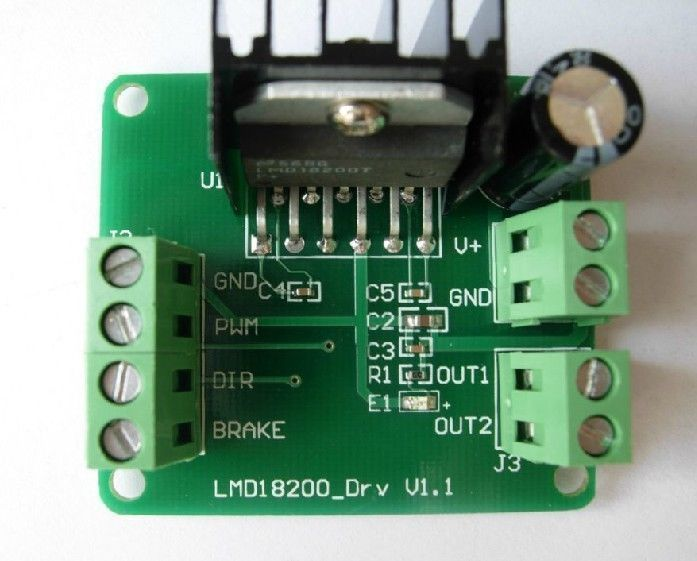
\includegraphics[scale = 0.3]{part/Proyecto_ejecutivo/memoria_constructiva/motor/img/modulopot}
		\caption{Módulo de potencia}\label{fig:Hbridge}
\end{figure}

\begin{figure}[H]
		\centering
		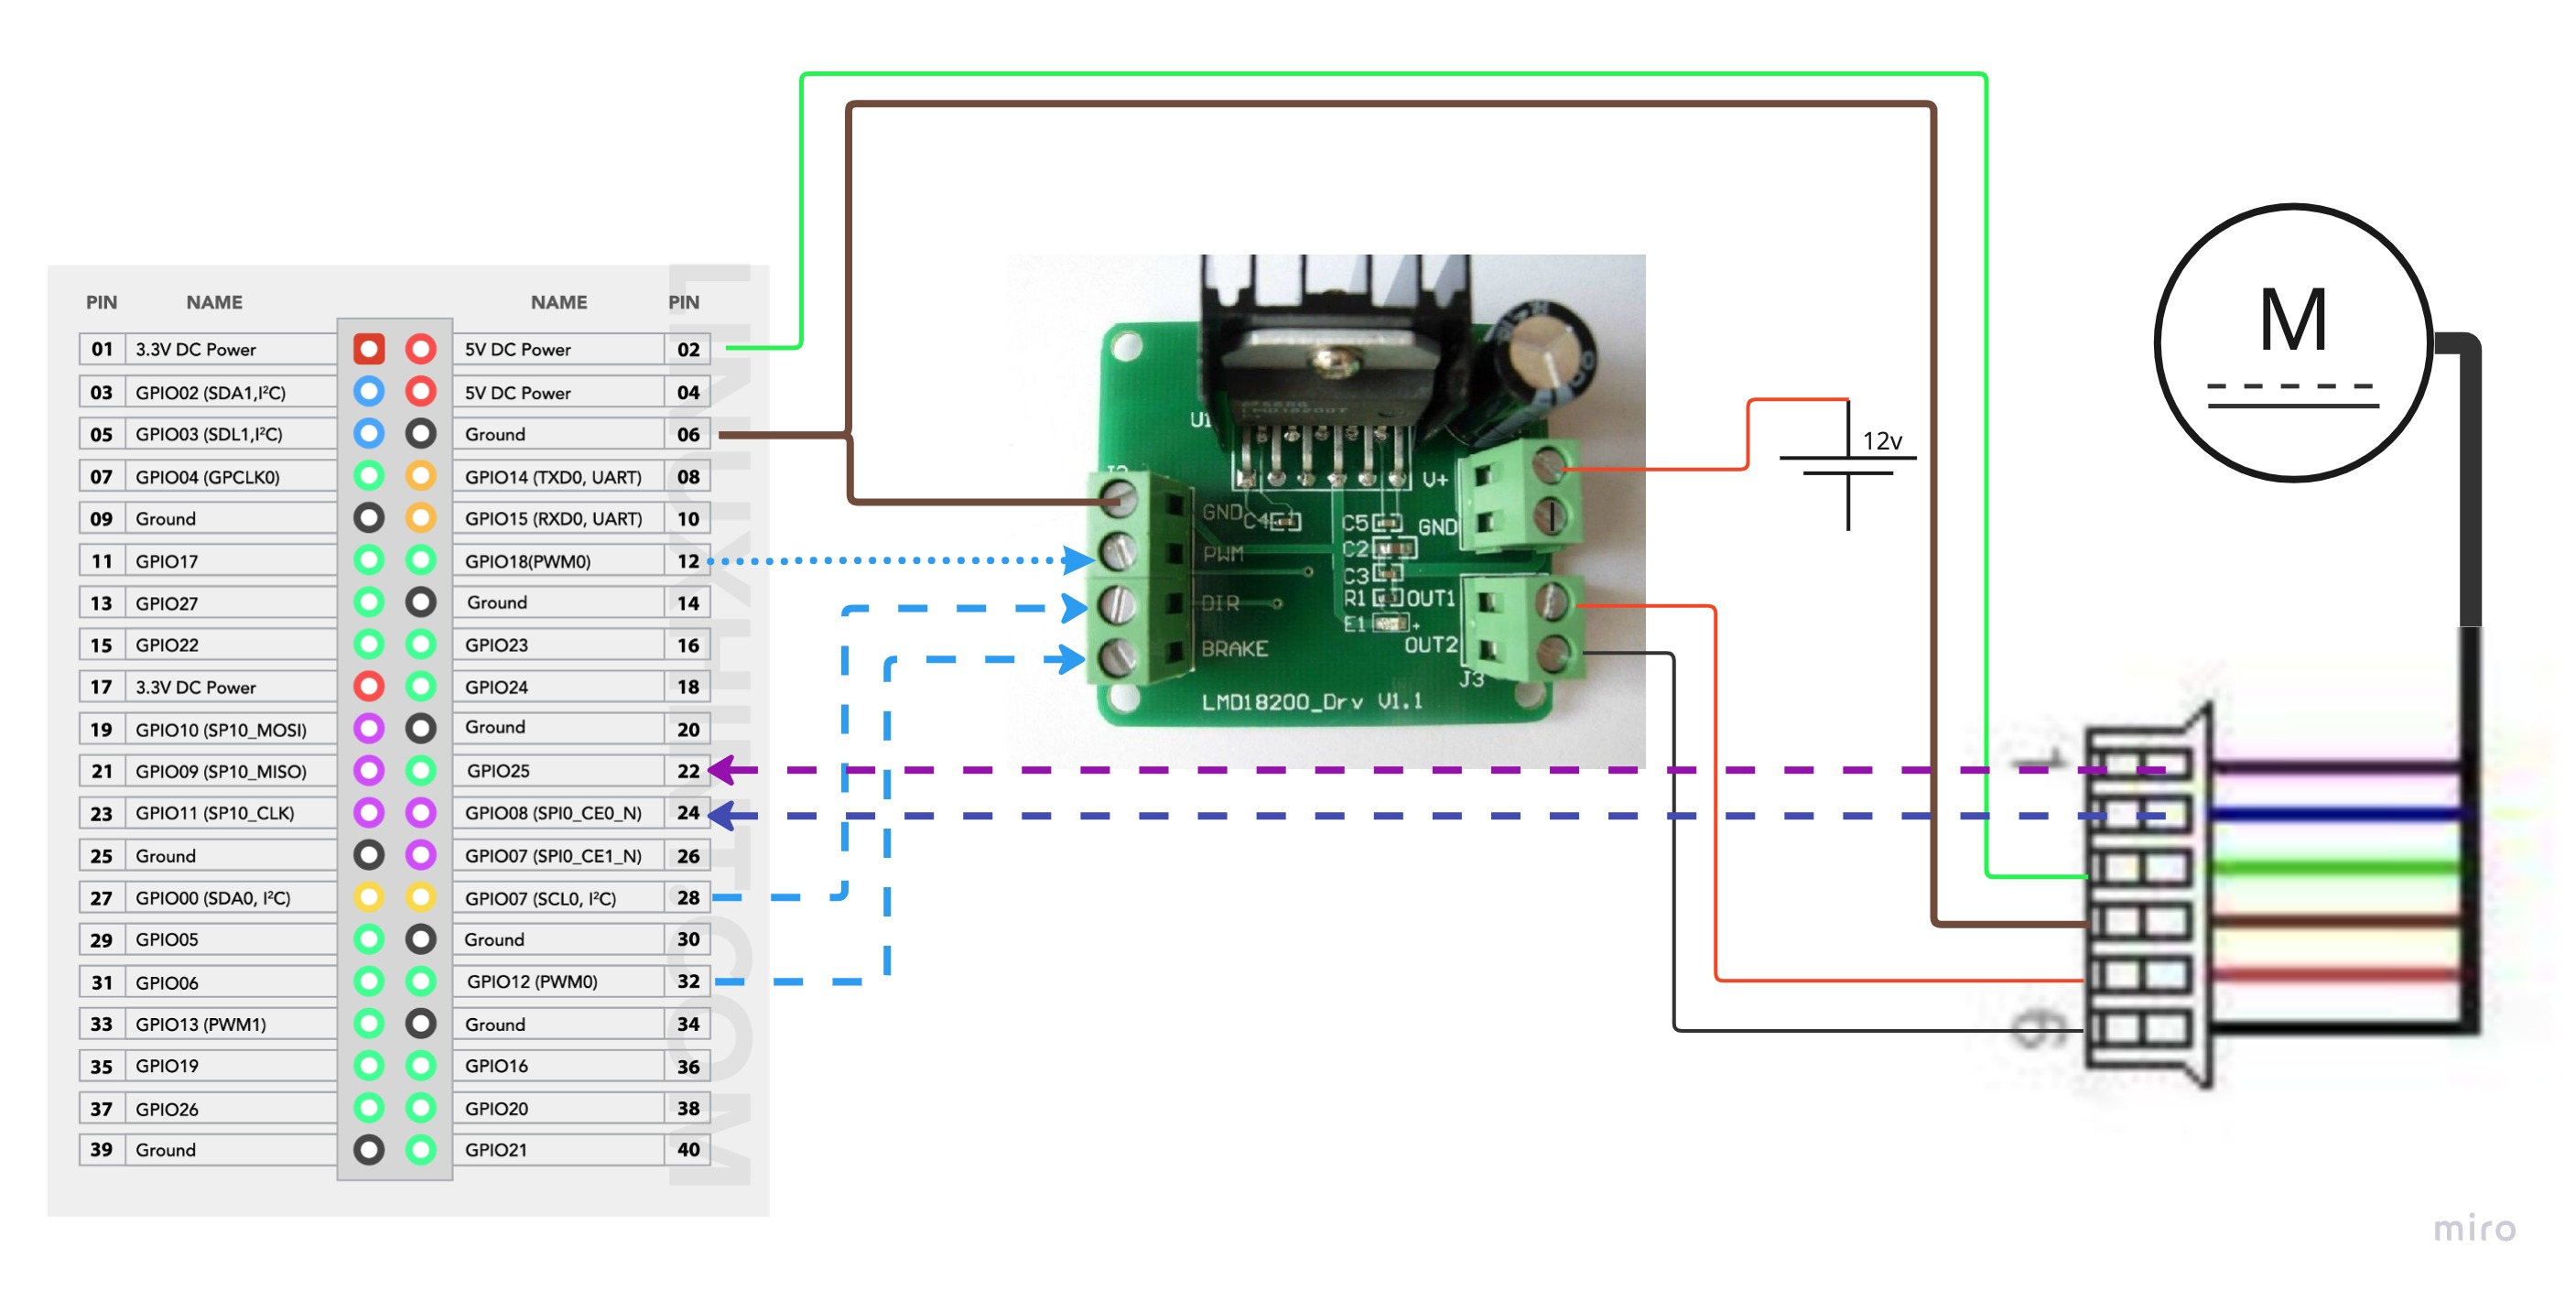
\includegraphics[scale = 0.15]{part/Proyecto_ejecutivo/memoria_constructiva/motor/img/connection diagram}
		\caption{Esquema de conexión hardware para el programa de control}\label{fig:conectionDiagram}
\end{figure}